\chapter{Конструкторская часть}

В данном разделе будут рассмотрены схемы вышеизложенных алгоритмов.

\section{Разработка алгоритмов}

На рисунке \ref{img:matrix} представлен матричный алгоритм поиска расстояния Левенштейна.

\begin{figure}[H]
	\begin{center}
		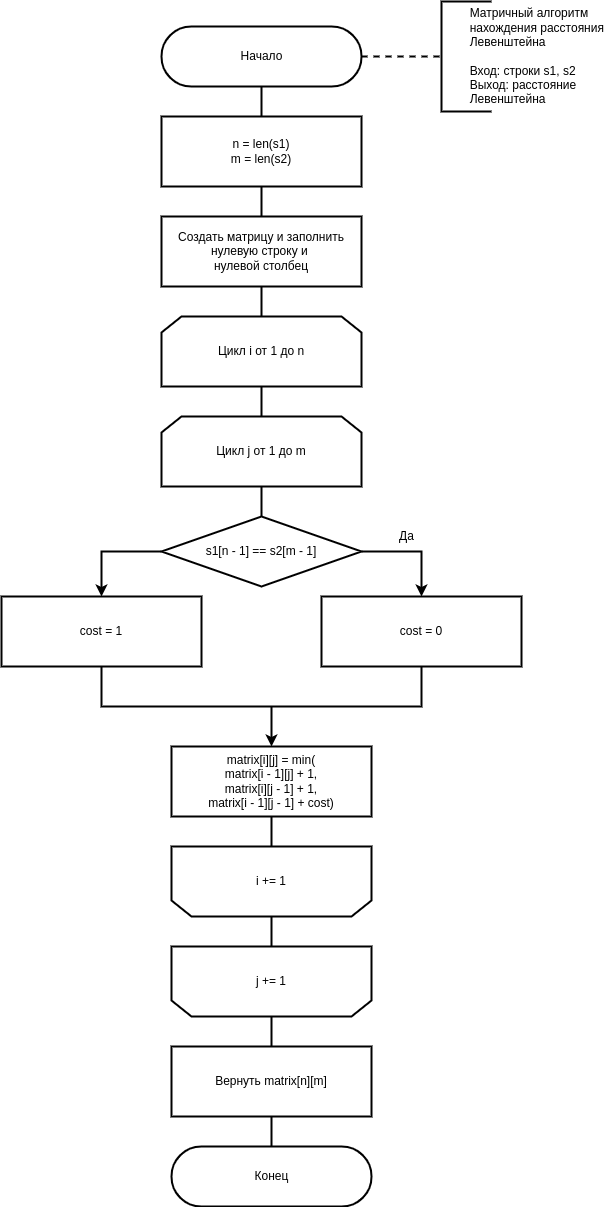
\includegraphics[scale=0.56]{img/matrix.png}
	\end{center}
	\captionsetup{justification=centering}
	\caption{Схема матричного алгоритма нахождения расстояния Левенштейна}
	\label{img:matrix}
\end{figure}

На рисунке \ref{img:dl_matrix} представлен матричный алгоритм поиска расстояния Дамерау-Левенштейна.

\begin{figure}[H]
	\begin{center}
		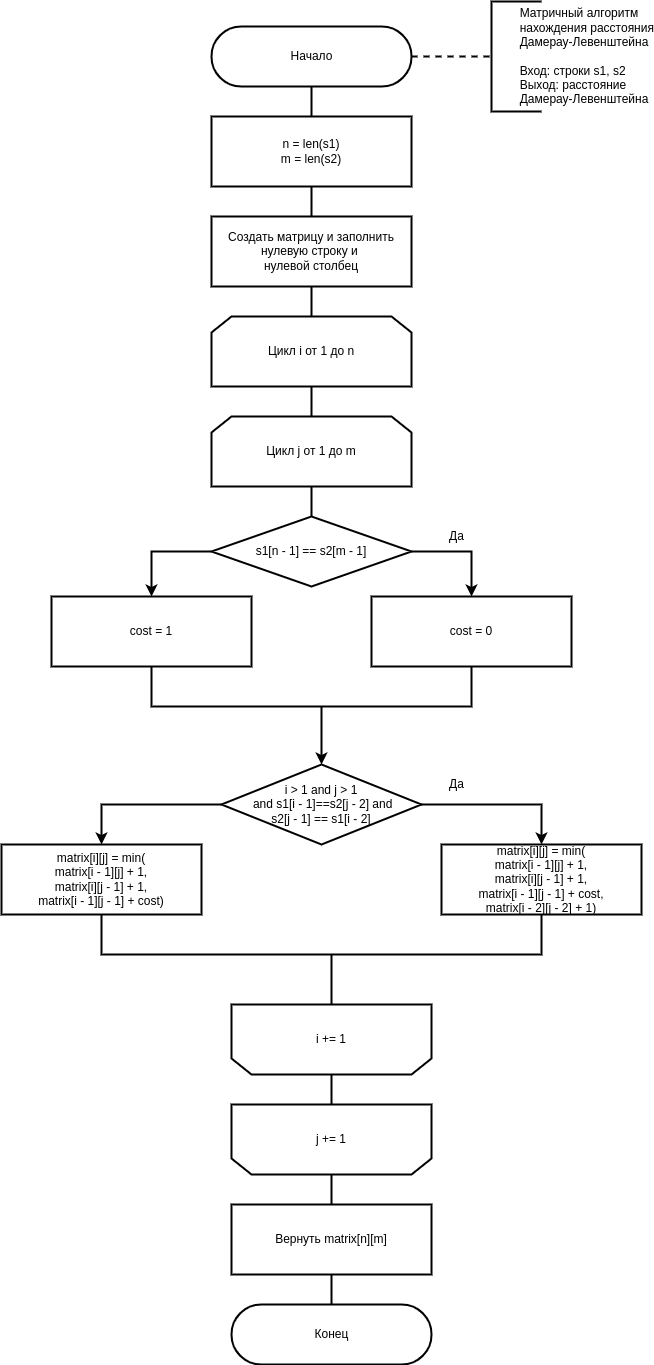
\includegraphics[scale=0.45]{img/dl_matrix.png}
	\end{center}
	\captionsetup{justification=centering}
	\caption{Схема матричного алгоритма нахождения расстояния Дамерау-Левенштейна}
	\label{img:dl_matrix}
\end{figure}

На рисунке \ref{img:dl_recursive} представлен рекурсивный алгоритм поиска расстояния Дамерау-Левенштейна.

\begin{figure}[H]
	\begin{center}
		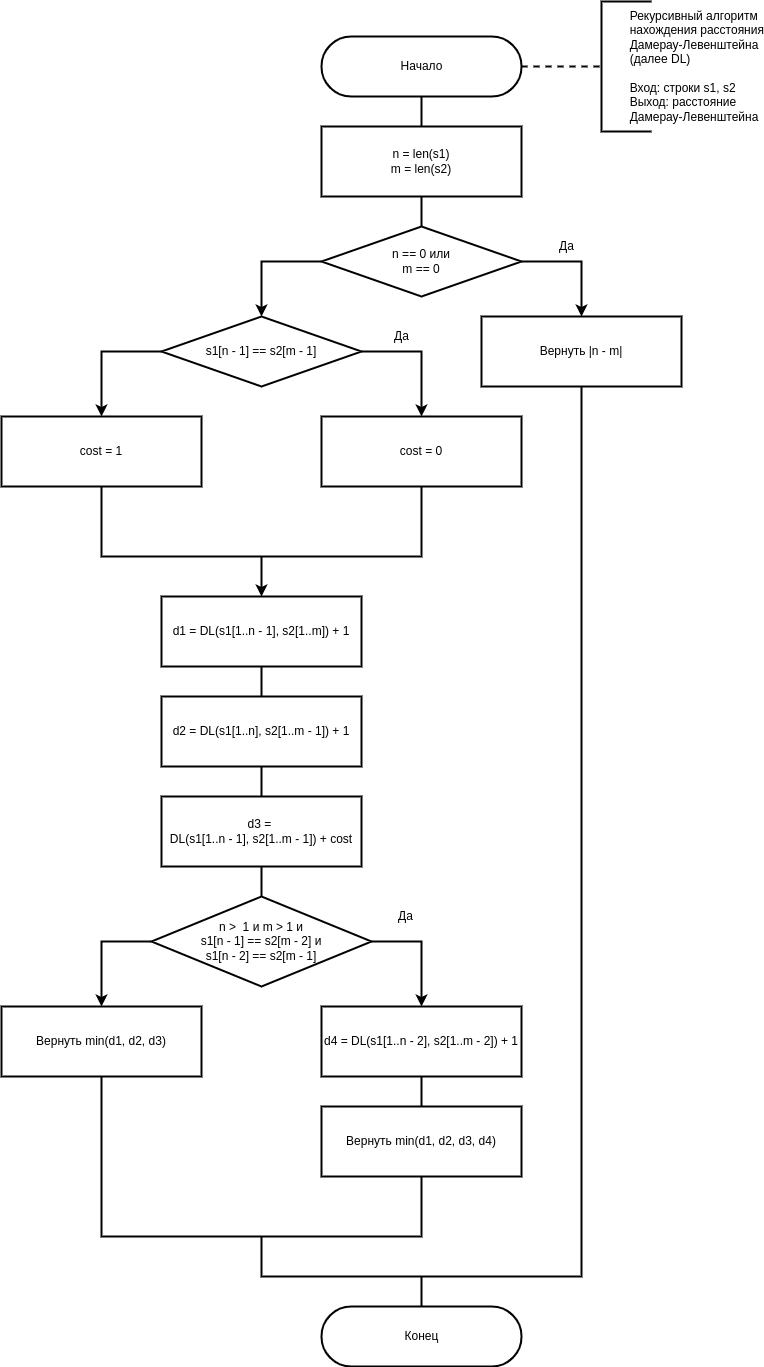
\includegraphics[scale=0.45]{img/dl_recursive.png}
	\end{center}
	\captionsetup{justification=centering}
	\caption{Схема рекурсивного алгоритма нахождения расстояния Дамерау-Левенштейна}
	\label{img:dl_recursive}
\end{figure}

На рисунке \ref{img:dl_recursive_cache} представлен рекурсивный алгоритм поиска расстояния Дамерау-Левенштейна с кешем.

\begin{figure}[H]
	\begin{center}
		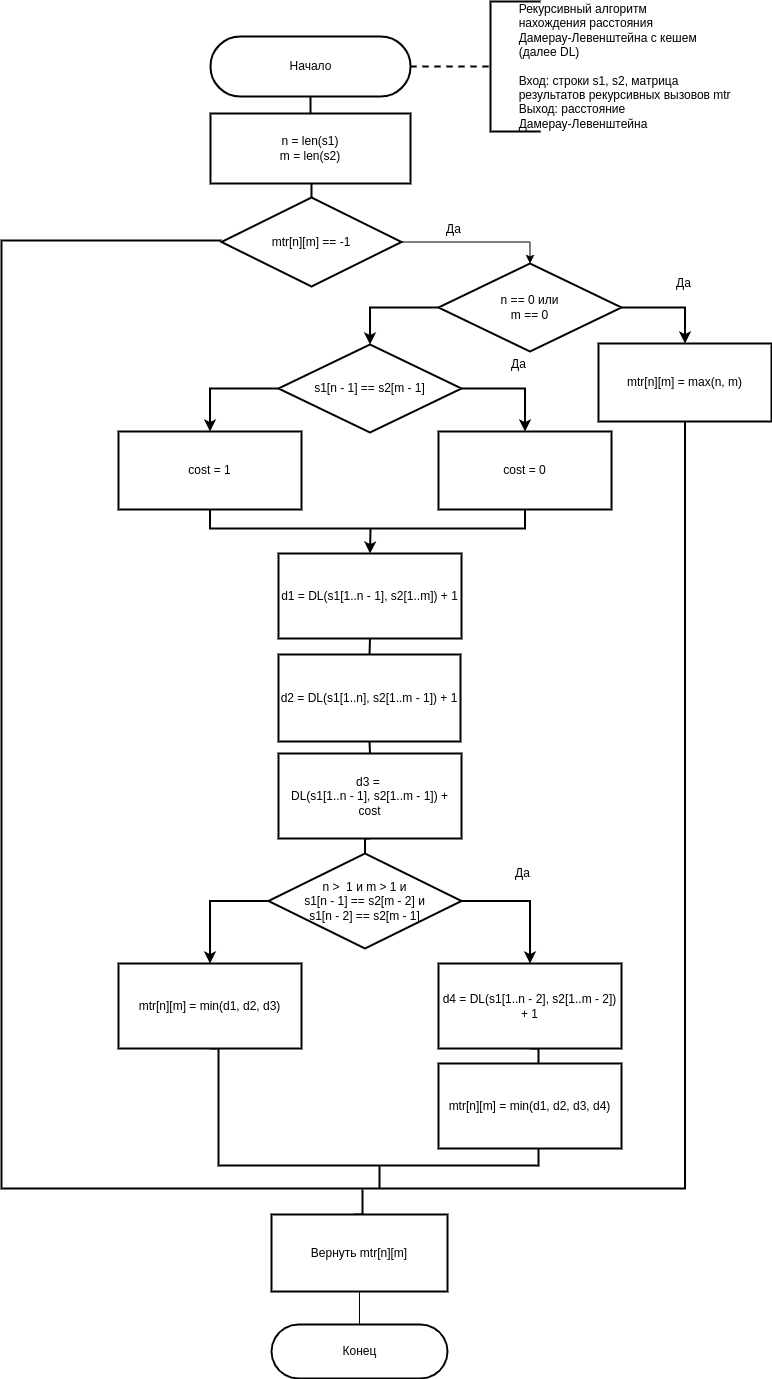
\includegraphics[scale=0.449]{img/dl_recursive_cache.png}
	\end{center}
	\captionsetup{justification=centering}
	\caption{Схема рекурсивного алгоритма нахождения расстояния Дамерау-Левенштейна с кешем}
	\label{img:dl_recursive_cache}
\end{figure}

\section*{Вывод}

На основе теоретических данных, полученных из аналитического раздела
были построены схемы требуемых алгоритмов.